\chapter{Guía de Uso}
\label{chap:guiauso}


	\section{Introducción}
	\gotrev{Última Revisión: 20-06-2012}
		
		Esta sección pretende mostrar una vista general de la aplicación y sus opciones. A lo largo de ella se explicarán todos los módulos del programa con los que el usuario puede interactuar y se detallará la función de determinados mecanismos.\\
		
		\begin{figure}[htbp]
		\centering
		\hspace*{-0.3in}
		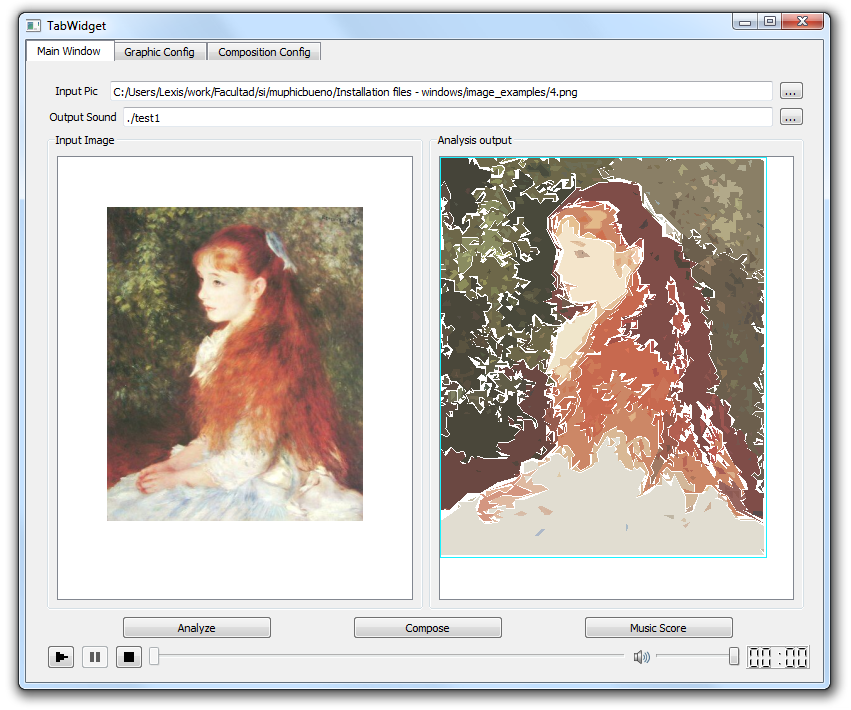
\includegraphics[scale=0.40]{graphics/interfazoverview.png}
		\caption{Vista general de la aplicación}
		\label{fig:interfazoverview}
		\end{figure}
		
		Como vemos en la Figura~\ref{fig:interfazoverview}, la aplicación dispone de tres pestañas: \emph{Main Window}, \emph{Graphic Config} y \emph{Composition Config}. La primera dispone de toda la funcionalidad necesaria para lanzar la aplicación, mientras que las otras dos aportan opciones para configurar el comportamiento del análisis y la composición.\\
		
		De forma general, todo usuario, experto o inexperto, se puede valer de la primera pestaña para usar la composición. Sin embargo, un usuario avanzado con conocimientos musicales y de qué tipos de análisis gráficos se realizan puede navegar por las pestañas restantes para configurar los procesos de composición y análisis de imagen, respectivamente.\\
		
		Se procede por tanto a explicar cada pestaña una por una.

	\section{Ventana principal}
	\gotrev{Última Revisión: 20-06-2012}
		
		Se encarga de la interacción básica con el usuario; muestra los resultados obtenidos y permite lanzar los principales componentes de la aplicación. 
		\\Esta compuesta por los siguientes elementos tal y como se puede ver en la Figura~\ref{fig:interfaz}:\\
		
		
		\begin{figure}[htbp]
		\centering
		\hspace*{-0.5in}
		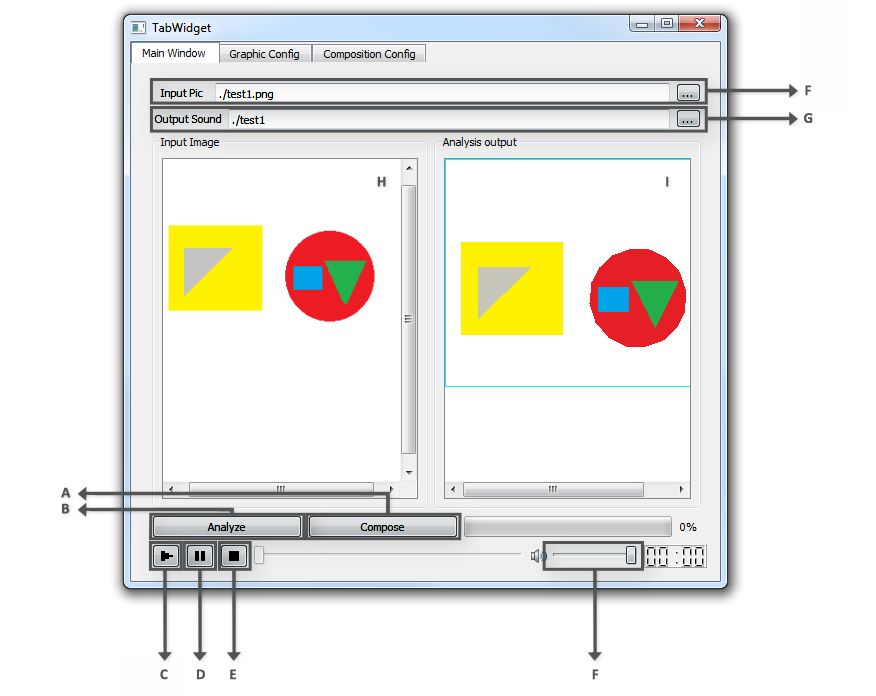
\includegraphics[scale=0.50]{graphics/interfaz.png}
		\caption{Vista general de la pestaña principal de la aplicación}
		\label{fig:interfaz}
		\end{figure}
		
		\noindent\textit{Carga de imagen de entrada [F]:} Permite al usuario elegir la dirección desde donde se cargará la imagen de entrada.\\
		
		\noindent\textit{Selección del archivo de audio de salida [G]:} Permite al usuario elegir la dirección donde se guardará el archivo de salida.\\
		
		\noindent\textit{Input Image [H]:} En este panel se muestra la imagen elegida para el análisis.\\
		
		\noindent\textit{Analysis output [I]:} En este panel se muestra el resultado del último análisis realizado pulsando el botón ``Analyze''.\\
		
		\noindent\textit{Botón Analyze [B]:} Tal y como su nombre indica, Analyze, realiza el analisis de la imagen pasada como parámetro de entrada. Tras analizarse, el resultado podrá observarse en el panel \textit{[I]}. Una vez pulsado el botón, y mientras dure el análisis, el botón pasará a mostrar el mensaje ``STOP'', pudiendo pulsarlo de nuevo para detener el análisis manualmente. Esta opción es bastante útil para imagenes grandes o complejas (con muchas variaciones de color que originan gran cantidad de formas), ya que el análisis puede tardar más de lo esperado y el usuario puede de esta manera detenerlo para luego relanzarlo con otra configuración más rápida.\\
		
		\noindent\textit{Botón Compose [A]:}\ Realiza la composición musical a partir de los datos analizados. Una vez compuesta la pieza musical, se podrá escuchar mediante los controles de control de sonido. Una vez pulsado el botón, y mientras dure el análisis, el botón pasará a mostrar el mensaje ``STOP', pudiendo pulsarlo de nuevo para detener la composición manualmente.\\
		
		\noindent\textit{Botón de Inicio de Reproducción [C]:} Permite al usuario iniciar la reproducción de la pieza musical compuesta previamente.\\
		
		\noindent\textit{Botón de Pausa de Reproducción [D]:} Pausa la pieza musical en reproducción.\\
		
		\noindent\textit{Botón de Detención de Reproducción [E]:} Detiene la reproducción completamente.\\
		
		\noindent\textit{Barra de sonido [F]:} Modifica el volumen de la reproducción en curso.

		
	\section{Configuración gráfica}
		\torev{Última revisión 13-06-12\\}
		En esta pestaña se encuentran todas las opciones relacionadas con el análisis de la imagen. En ella se podrán configurar opciones que hagan que el proceso de análisis varíe en velocidad, precisión o estilo.\\
		
		De entre los parámetros de configuración, existen los llamados ``generales'', que siempre aparecen visibles al usuario, y los ``específicos'', que complementan a los generales y sólo aparecen cuando el contexto lo especifica. En la Figura~\ref{fig:interfazgraphic} podemos ver detalladamente los parámetros generales.\\
		
		\begin{figure}[htbp]
		\centering
		\hspace*{-0.5in}
		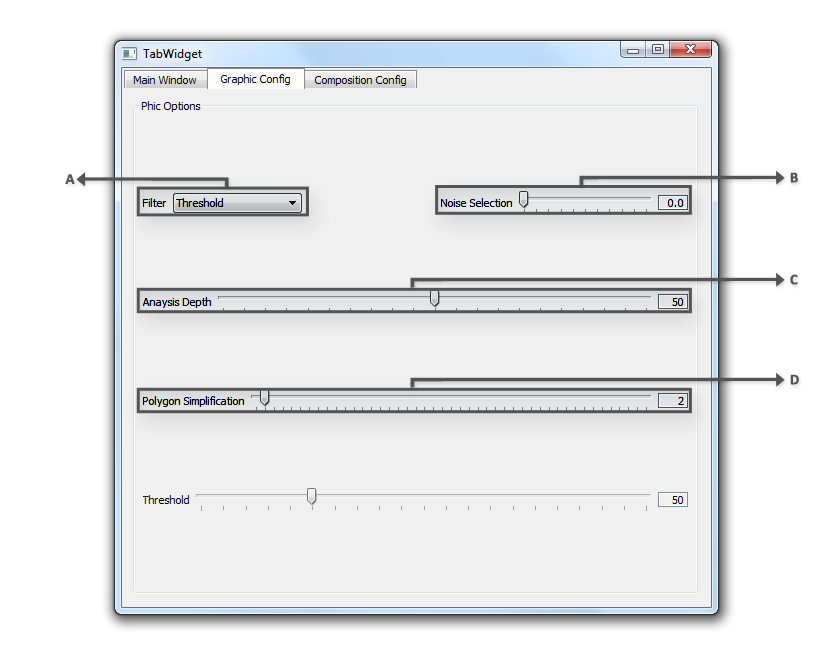
\includegraphics[scale=0.5]{graphics/interfazgraphic.png}
		\caption{Vista general de la pestaña de configuración gráfica}
		\label{fig:interfazgraphic}
		\end{figure}
		
		\noindent\textit{Tipo de filtrado de imagen [A]:} Distintos filtros en la imagen producirán diferentes formas de entender las formas que hay en ellas. De forma un poco más precisa, pero sin llegar a entrar en detalles técnicos, los filtros se encargan de transformar la imagen original a un mapa de bits en blanco y negro, que posteriormente se analizará para detectar polígonos en él. Un buen filtro diferenciará las deseadas superficies de color como manchas blancas independientes.\\
		
		\noindent\textit{Selección de ruido [B]:} Mediante esta barra el usuario puede elegir el tamaño mínimo de las formas por debajo del cual no se considerarán relevantes en el análisis. El valor representa un porcentaje respecto al área total de la imagen, de forma que un valor $n$ de Selección de Ruido determina que todas las formas con área menor a un $n$\% del área total de la imagen se considerarán ruido y no serán estudiadas.\\
		
		\noindent\textit{Profundidad del análisis [C]:} Permite variar el nivel de detalle con el que se realizará el análisis, o para ser más precisos: determina el número de píxeles respecto del total que se tienen en cuenta para el anális. Un valor grande de profundidad hará que el análisis se realice examinando la mayor parte de los píxeles de la imagen (se establece como restricción que nunca se examinen más de 1000x1000 píxeles, por cuestiones de optimización), mientras que un valores pequeños aumentarán la velocidad del proceso a costa de tener en cuenta menos píxeles en la imagen.\\
		
		\noindent\textit{Simplificación de polígonos [D]:} Una vez detectadas las formas de color, es necesario que se aproximen a una lista de vértices para reducir el peso de la información sin modificar la carga de la misma. El nivel de fidelidad en la transformación de formas a polígonos se establece con este parámetro: un valor alto determina una gran fidelidad a costa de mayor tiempo de análisis, y viceversa.\\

		
		\vspace{0.2in}Los parámetros ``específicos'' dependen única y exclusivamente del tipo de filtro seleccionado [A], ya que cada tipo de filtro introduce nuevas opciones que configurar. \\
		
		Todo filtro en la aplicación que nos ocupa, como ya se comentó anteriormente, realizan la misma función: detectar formas y expresarlas como superficies blancas. A continuación se explica de forma general el funcionamiento de cada filtro y sus parámetros ``específicos''.\\
		
	\noindent\textbf{Threshold}\\
		
		Este filtro, contenido en varias librerías de procesado de imágenes (ver \cite{opencvDoc}), transforma la imagen a escala de grises para luego marcar como blancos todos los píxeles con un valor de gris superiores a un umbral dado, y como negros el resto (una explicación más formal se puede encontrar en \cite{pajares}).\\
		
		Los parámetros específicos que usa son:\\		
		
		\noindent\textit{Valor del umbral:} Establece el valor del umbral antes explicado.\\
		
	\noindent\textbf{Adaptive Threshold}\\

		Mientras que el filtro anterior utiliza un mismo umbral para toda la imagen, Adaptative Threshold (ver implementación en \cite{opencvDoc}, y su descripción formal en \cite{pajares}) usa un umbral distinto para diferentes regiones de la imagen, en función de los valores de los píxeles tratados.\\ 
		
		Este filtro no usa parámetros específicos, ya que modifica el valor del umbral cada vez que le resulta necesario.\\
		
	\noindent\textbf{Canny}\\

		Utiliza el algoritmo de detección de regiones del mismo nombre, desarrollado en 1986 por John F. Canny (ver implementación en \cite{opencvDoc}, y una descripción detallada en \cite{pajares}). Una vez encontrados los bordes, establece las figuras que estos delimitan.\\
		
		Este filtro no usa parámetros específicos.\\
		
	\noindent\textbf{Hue Division}\\


		Se trata de un filtro propio que busca asocia manchas de color con conjuntos de píxeles vecinos con valores RGB dentro de un mismo rango de rojo (R), azul (B) y verde (G). Los parámetros específicos son:\\
		
		\noindent\textit{Niveles de color:} Este parámetro determina el número de intervalos posibles de color que puede haber en cada canal de color, y por tanto determinará la amplitud de cada rango. Un valor igual a 3 indica que un píxel cualquiera puede entrar dentro de 3 intervalos posibles en el canal rojo, otros 3 en el azul y otros 3 en el verde. De esta forma cada píxel entra dentro de una de las $3*3*3=27$ categorías de color, simplificando el análisis. Un valor muy grande de este parámetro hará que haya más categorías de color y que por tanto colores que antes se consideraban parte de una misma forma ahora se consideren como parte de formas independientes con colores más específicos. Un valor muy pequeño hará que se interpreten formas más amplias (incluyendo píxeles más diversos).\\
		
	\noindent\textbf{Color Threshold}\\

		Se trata de un filtro propio que adapta el filtro Threshold para una imagen de 3 canales. En vez de considerar como figuras aquellas agrupaciones de píxeles cuyos valores en escala de grises sean inferiores a un umbral, considera aquellas que en su canal de Matiz (Hue), Saturación (Saturation) y Valor (Value) sean menor que un umbral, originando cada canal formas independientes.\\
		
		Los parámetros específicos de este filtro determinarán el valor de los umbrales de cada canal determinado en formato de imagen HSV.\\		
		
		\noindent\textit{Valor del umbral de Matiz}\\
		\noindent\textit{Valor del umbral de Saturación}\\
		\noindent\textit{Valor del umbral de Valor}

		
		\color{blue}
		
		\vspace{0.5in}Para dar una vista general de las características y formas de trabajar de cada filtro de análisis, se muestran en la Figura~\ref{fig:analresults} los resultados que proporciona cada uno de ellos para una misma imagen de entrada. Todos ellos han usado como valores de entrada comunes los siguientes:

		
		\begin{center}
			Noise Selection $= 0$\\
			Analysis Depth $= 100$\\
			Polygon Simplification $= 1$\\
		\end{center}
		
			\begin{figure}[htbp]
			\centering
			\hspace*{-0.0in}
			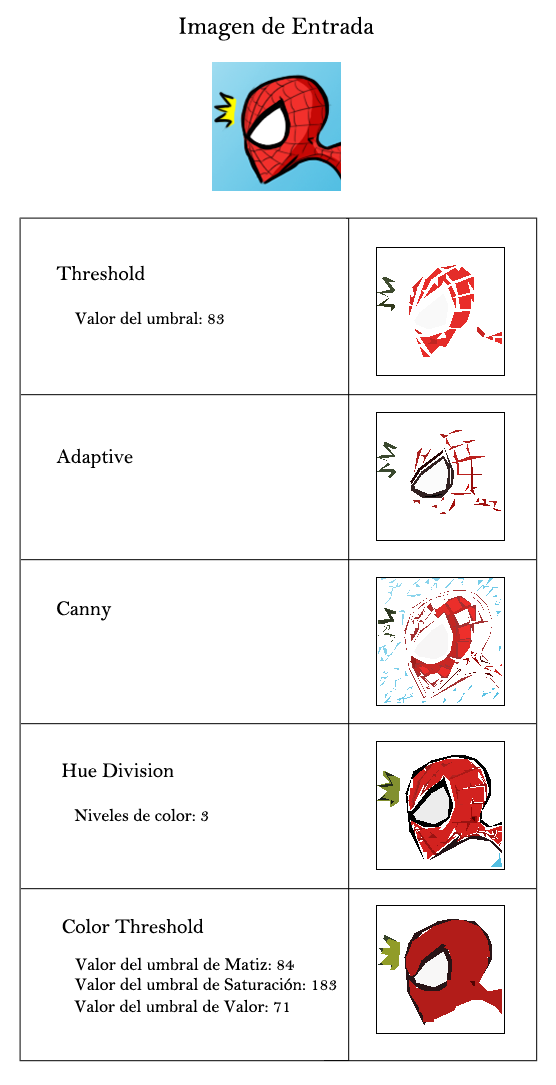
\includegraphics[scale=0.5]{graphics/analresults.png}
			\caption{Tabla con las distintas salidas de cada filtro de análisis}
			\label{fig:analresults}
			\end{figure}
		
		
		Como se puede observar, el filtro Hue Division es el más fiel de los cinco, captando en la representación de la imagen la mayor parte de la información que había en la imagen de entrada.		\color{black}

		
		\section{Configuración de composición}
		\gotrev{Última Revisión: 20-06-2012}
		
		Esta pestaña contiene todos los parámetros que se pueden configurar relativos a la composición algorítmica. Estos, como muestra la Figura~\ref{fig:interfazcomp} son:\\
		
		\begin{figure}[htbp]
		\centering
		\hspace*{-0.5in}
		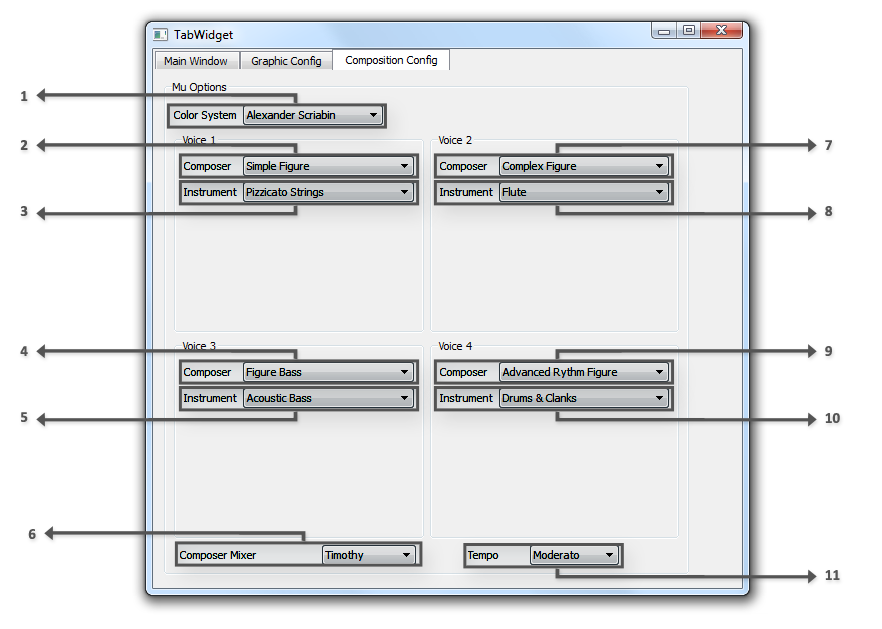
\includegraphics[scale=0.5]{graphics/interfazcomp.png}
		\caption{Vista general de la pestaña de configuración gráfica}
		\label{fig:interfazcomp}
		\end{figure}
		
		\noindent\textit{Sistema de color[A]:} Permite alternar entre las diferentes relaciones tono-color explicadas en la Sección~\ref{sec:algComposicion}.\\
		
		\noindent\textit{Algoritmo de composición para la primera voz[B]:} Con esta opción, el usuario puede elegir, de entre los distintos algoritmos de composición, el que se usará para que generar la melodía principal.\\
		
		\noindent\textit{Algoritmo de composición para la segunda voz[G]:} Con esta opción, el usuario puede elegir, de entre los distintos algoritmos de composición, el que se usará para que generar la segunda melodía principal.\\

		\noindent\textit{Algoritmo de composición para la tercera voz[D]:} Con esta opción, el usuario puede elegir, de entre los distintos algoritmos de composición del bajo, el que se usará para que generar el bajo armónico.\\
		
		\noindent\textit{Algoritmo de composición para la cuarta voz[I]:} Con esta opción, el usuario puede elegir, de entre los distintos algoritmos de composición de ritmos, el que se usará para que generar el ritmo de la pieza musical final.\\
		
		\noindent\textit{Selección de instrumentos [C], [H], [E] y [J]:} Permiten seleccionar los instrumentos con los que sonaran las distintas voces.\\

		\noindent\textit{Algoritmo de composición general[F]:} Determina qué algoritmo se usará para recorrer la imagen y aplicar los algoritmos de las distintas voces. Se explica con detalle en la Sección~\ref{sec:algComposicion}.\\

		\noindent\textit{Tempo[K]:} Como su nombre indica, su valor determina el tempo con el que sonará la pieza musical compuesta.\\
		
	\section{Requisitos de instalación}
	\label{sec:reqinstalacion}
	\gotrev{Última Revisión: 20-06-2012}
	
		Muphic es una aplicación multiplaforma con soporte para Linux y Windows de 32 y 64 bits, siendo en ambos una aplicación portable. Para finalizar este capítulo, se detallará a continuación las peculiaridades de ejecución en cada plataforma.
		
		\subsection{Windows}
		
		Para ejecutar la aplicación basta con descomprimir el archivo descargado y ejecutar la aplicación.
		
		\subsection{Linux}
		
		Para utilizar la aplicación en cualquier distribución de Linux, habrá que descomprimir el archivo y generar los ejecutables con la herramienta make. Ciertos elementos del sistema (la interfaz gráfica y los controles de reproducción de sonido) requieren que el usuario tenga instaladas ciertas librerías que no se incluyen en la descarga de la aplicación. Estos paquetes son:
		
		\begin{itemize}
			\item Librerías de qt versión 4.7.4, disponibles en su página web (ver \cite{qtlibs}).		
			\item \emph{libphonon-dev (multimedia framework from KDE-development files)} 
			\item \emph{libphonon4 (multimedia framework from KDE-core library)}
			\item \emph{phonon (multimedia framework from KDE-metapackage)}
			\item \emph{phonon-backend-gstreamer (Phonon GStreamer 0.10.x backend)}
			\item \emph{libqtscript4-phonon (Qt Script bindings for the Qt 4 Phonon library)}
			
		\end{itemize}
	
		Si el paquete \emph{phonon-backend-gstreamer}, por cualquier razón, fuera el origen de algún fallo; el usario puede elegir probar con otros tipos de backend, como por ejemplo \emph{phonon-backend-vlc}.